\begin{problem}{1}
	\textbf{Real space and nonlinear divergence}

  As $k$ increases, the pendulum's trajectory becomes less linear. The numerical
  solutions also diverge after a number of periods. The 3rd order symplectic
  method diverges at $k ~ 15$, and the semi-implicit Euler's method diverges at
  $k ~ 18.5$.

\noindent
\begin{figure}[ht!]
	\centering
	\begin{minipage}[b]{0.4\textwidth}
	  \includegraphics[scale=0.6]{../figures/k3_nonlin.pdf}
	\end{minipage}
	\hfill
	\begin{minipage}[b]{0.4\textwidth}
	  \includegraphics[scale=0.6]{../figures/k9_nonlin.pdf}
	\end{minipage}
	\begin{minipage}[b]{0.4\textwidth}
	  \includegraphics[scale=0.6]{../figures/k15_nonlin.pdf}
	\end{minipage}
	\hfill
	\begin{minipage}[b]{0.4\textwidth}
	  \includegraphics[scale=0.6]{../figures/k17_nonlin.pdf}
  \end{minipage}
	\caption{Real space for various $k$}
\end{figure}
\end{problem}
\begin{problem}{2}
	\textbf{Total energy over time}

  Although the total energy oscillates over time, the amplitude of the
  oscillation is small. More importantly, the energy does not diverge over time.
  All plots are with $\delta t = 0.1$

\begin{figure}[ht!]
  \centering
	  \includegraphics[scale=0.6]{../figures/energy_time.pdf}
	\caption{Real space for various $k$}
\end{figure}
\end{problem}

\begin{problem}{3}
	\textbf{Comparing 3rd order symplectic integrator with semi-implicit Euler's in error over time}

  At first, the left of figure \ref{error} appeared a surprise as the
  semi-implicit Euler's method seem to converge to the analytical method over
  time. However, with longer time, the right plot reveals that the semi-implicit
  Euler's has a periodic error, and the 3rd-order symplectic method has an error
  that grows much slower over time. We integrate over the square of error with
  regard to the analytical solution to measure the total error.

\begin{figure}[ht!]
	\centering
	\begin{minipage}[b]{0.4\textwidth}
	  \includegraphics[scale=0.6]{../figures/error-10.pdf}
	\end{minipage}
	\hfill
	\begin{minipage}[b]{0.4\textwidth}
	  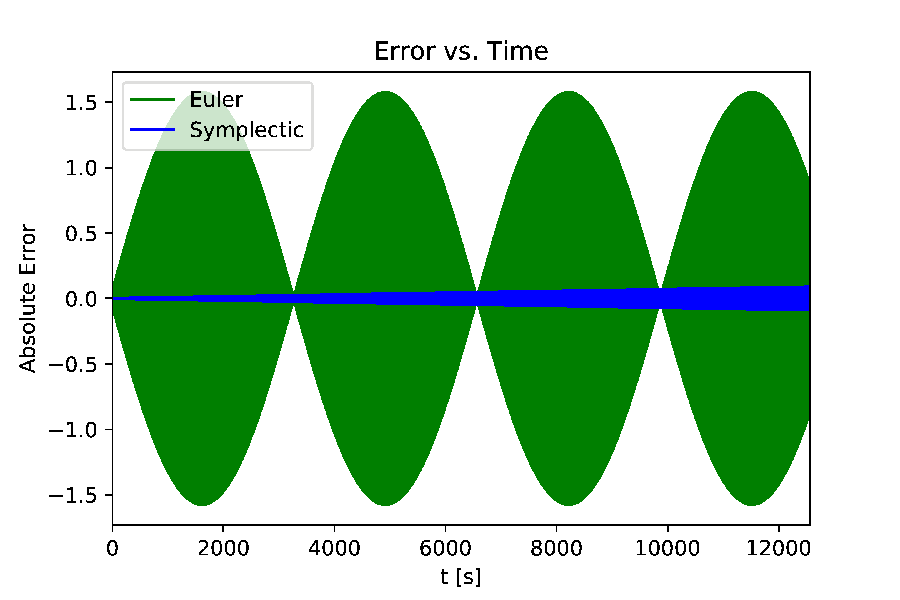
\includegraphics[scale=0.6]{../figures/error-4k.pdf}
	\end{minipage}
	\caption{Real space for various $k$}
  \label{error}
\end{figure}
\end{problem}
